% !TEX root = ../../../main/aws_chabauty.tex
\newpage
\section{David Zureick-Brown: Effective Chabauty}
\subsection{Lecture 1}

\noindent Lorenzini-Tucker \par
\noindent McCollem-Poonen \par
\noindent Stoll \par
\noindent Katz-ZB \par\vspace{2\baselineskip}


\begin{thm}[K-ZB]
Let $X/\Q$ be a `nice' curve with $r= \rank J(\Q)$, and $p>2r+2$ a prime. Let $\fX$ be a regular proper minimal model of $X$. Let $r<g$, then 
	\[
	\#(X(\Q)) \leq \# \fX_{\F_p}^?(\F_p) + 2r
	\]
\end{thm}


\begin{thm}[Coleman, ``rank favorable bound'']
In the situation above, 
	\[
	\#(X(\Q)) \leq \# \fX_{\F_p}^?(\F_p) + (2g-2)
	\]
\end{thm}


A question of Mazur is can we bound $\#X(K)$ using the rank of $J(K)$ and $g$?


\begin{conj}[Uniformity Conjecture]
There exists $B(K,g)$ such that for all nice $X/K$ of genus $g$ with
	\[
	\#X(K) \leq B(K,g)
	\]
\end{conj}


Work of Poonen et al gives heuristics that, in the case of $X$ an elliptic curve, imply $r$ is bounded. 


The Weak Lang Conjecture states that if $X/K$ is a variety of general type, then there is $Z \subseteq X$ closed such that $Z(K) \subseteq X(K)$. 


\begin{thm}[Caparso,Harris,Mazur]
The Weak Lang Conjecture implies the Uniformity Conjecture
\end{thm}


\begin{ex}[Gordon-Grant, '93]
Let $X: y^2= x(x-1)(x-2)(x-5)(x-6)$. This is a hyperelliptic curve with $g= 2$ and rank 1. But $r=1 < 2$ so Coleman applies. Then $\#X(\Q)= 10$ GWP, 3 IG and IQ $\pm 120$. But mod 7, we have $\#X(\F_7)= 8$ gWP, $(3, \pm 6)$. 
	\[
	10 \leq \#X(\Q) \leq \#X(\F_7) + 2 = 8+2= 10
	\]
\end{ex}


\begin{thm}[Stoll]
Suppose that $X$ is hyperelliptic, and suppose that $r \leq g-3$. Then $\#X(\Q) \leq 3(r+4)(g-1) + \max\{1,4r\} \cdot g$.
\end{thm}


\begin{thm}[Katz-Rabinoff-ZB]
Suppose $r \leq g-3$. Then $\#X(\Q) \leq 84 g^2 - 98g + 28$. 
\end{thm}



% Effective Manin-Mumford
\subsubsection{Effective Manin-Mumford}

Let $X$ be a curve and $X \stackrel{i}{\hra} J$. Then $\#i(X) \cap J_\tor < \infty$, proven by Raynaud, Buildum, Coleman.

	\[
	X \hra J \ma{\log} \lie J
	\]
Then the integrals vanish on $X \cap J_\tors$. The nice thing here is that there is no necessary rank condition. 


\begin{thm}[KRZB]
\begin{itemize}
\item $(X \cap J_\tors)(\Q) \leq (?)$
\item $I$ and $X$ is very degenerate, e.g. totally degenerate
\end{itemize}
then we can bound $\# \cap J_\tors \leq ---$
\end{thm}


	\begin{figure}[!ht]
	\centering
	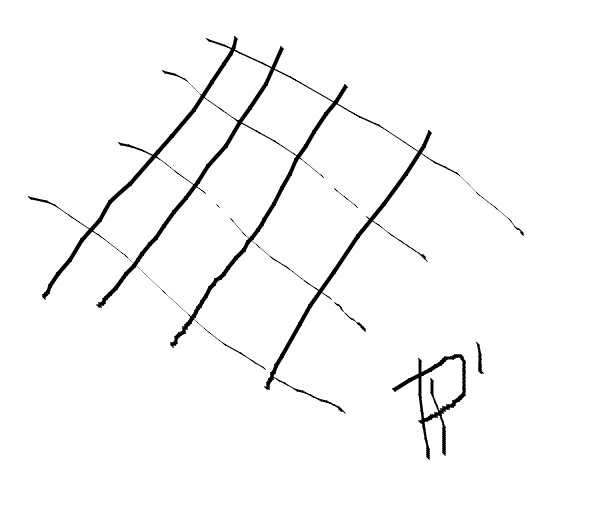
\includegraphics[width=0.3\textwidth]{../images/im2.png}
	\end{figure}
	
%	\begin{figure}[!ht]
%	\centering
%	\begin{tikzpicture}
%	\begin{axis}[
%	hide axis,
%	xmin=0, xmax=5,
%	ymin=0, ymax= 5
%	%rotate=45
%	]
%	\foreach \s in {-2,-1,0,1,2,3,4} {%
%		\addplot[domain=0:3,samples=50,black,thick] ({\x},{2-2*\x-\s}); 
%		\addplot[domain=0:3,samples=50,black,thick] ({\x},{2*\x+\s-4});
%	}
%	\end{axis}
%	\end{tikzpicture}
%	\end{figure}
	
	
	\[
	\begin{tikzcd}
	X(\Q) \arrow[hook]{r} & X(\Q_p) \arrow[hook]{d} \arrow{dr} \\
	J(\Q) \arrow[hook]{r} & J(\Q_p) \arrow{r}{\log} &  \lie J_{\Qp}
	\end{tikzcd}
	\]
where the log map is $D \mapsto (\omega \mapsto \int_Q^D \omega)$


`Black box Chabauty'.

\begin{itemize}
\item Setup
\item local analysis
\item global coordination 
\end{itemize}


Setup

Let $r<g$. There exists $V \subseteq H^0(X_{\Q_p}, \Omega^1)$ such that for all $P,Q \in X(\Q)$, $\int_P^Q \omega= 0$ for all $\omega \in V$ and $\dim V \geq g-r > 0$.


Local Analysis:

We can compute $\int_P^Q \omega$ locally and analyze with a Newton Polygon.

	\begin{figure}[!ht]
	\centering
	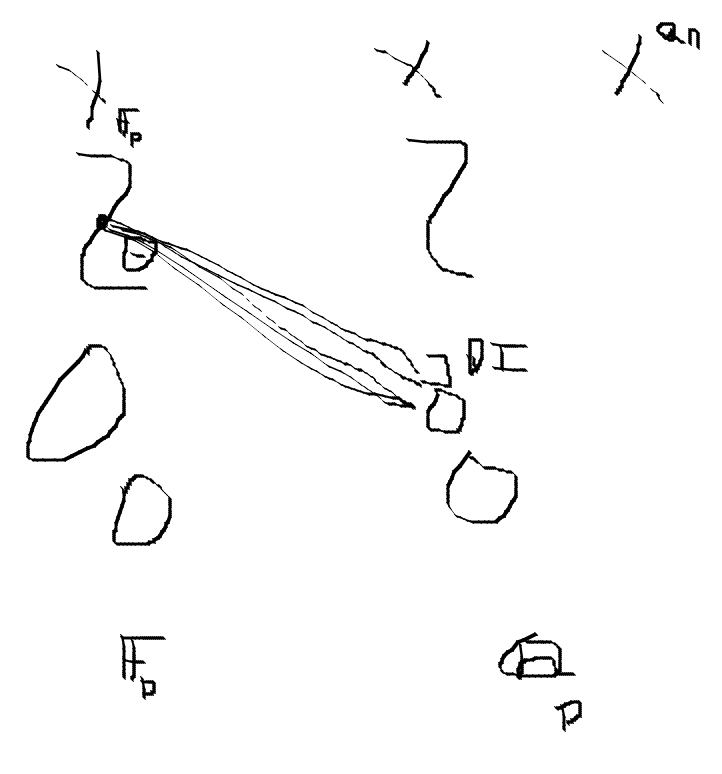
\includegraphics[width=0.3\textwidth]{../images/im3.png}
	\end{figure}

$[QI:= \{P \in X(\Q_p)$ such that $P \equiv Q \mod p \} \simeq p\Z_p$, the $p$-adic disc. Where the map is $p \mapsto u(P)$, where $u$ is a uniformizer at $\tilde{Q}$, a lift of $Q$.


\begin{ex}[HP survey]
$X: y^2= f(x)= x^6+8x^5+\cdots+1= xg(x)+1$.

$(0,1) \in X(\F_3)$.

$[(0,1)] \ma{\sim} p\Z_p$ with map $p \mapsto X(P)$ forward and $t \mapsto (t,\sqrt{tg(t)+1})$, which converges because $t$ is small, $\nu_p(t) > 0$. 
\end{ex}


To compute $\int_P^Q \omega$, only compute ``tiny'' integrals, i.e. $P=Q \mod p$. If $Q \in [P] \simeq p \Z_p \ni t$ with $\omega |_{[P]} = f(t) \;dt$ for some $f(t) \in \Z_p[1+1]$.
	\[
	\int_P^Q \omega= \int_Q^t f(t) \;dt = I(t)
	\]
integrating formally. 

























